\documentclass[../poliXuniversity_hospital_-USP-report.tex]{subfiles}
\graphicspath{ {images/}{../images/}{../../images/} }
\begin{document}
\clearpage

\section{Sinalização}

A placa de Sinalização é a mais importante esteticamente para o robô. Ela foi idealizada, desde da primeira versão do robô hospitalar, para realizar a iluminação e comunicação por luz (como faróis). De maneira geral ele controla uma série de leds rgbs endereçáveis e strobos automotivos. Além de, claro, como já mencionado antes, enviar e receber informações da placa de controle principal.

\subsection{Placa}

Como módulo, existem muitas minúcias que precisamos tomar ao projetá-las. A placa de Sinalização, para segunda versão do robô hospitalar, com objetivo de evitar problemas e realizar testes, teve duas versões: um protótipo, que já foi finalizado, e uma versão oficial, ainda em desenvolvimento. 

%================================ SINALIZAÇÂO PROTÒTIPO========================
\subsubsection{Protótipo}

O protótipo da placa de Sinalização foi refeito uma única vez. Como se trata de uma placa fresada, pode ser refeita no próprio laboratório do professor orientador. O projeto da placa eletrônica, assim como o de todos os módulos, foi dividido em esquemático e Printed Circuit board (PCB)  ou placa de circuito impresso.

\begin{figure}[!h]
\centering
    \caption{Protótipo placa de Sinalização - Esquemático principal }
    \centering % para centralizarmos a figura
    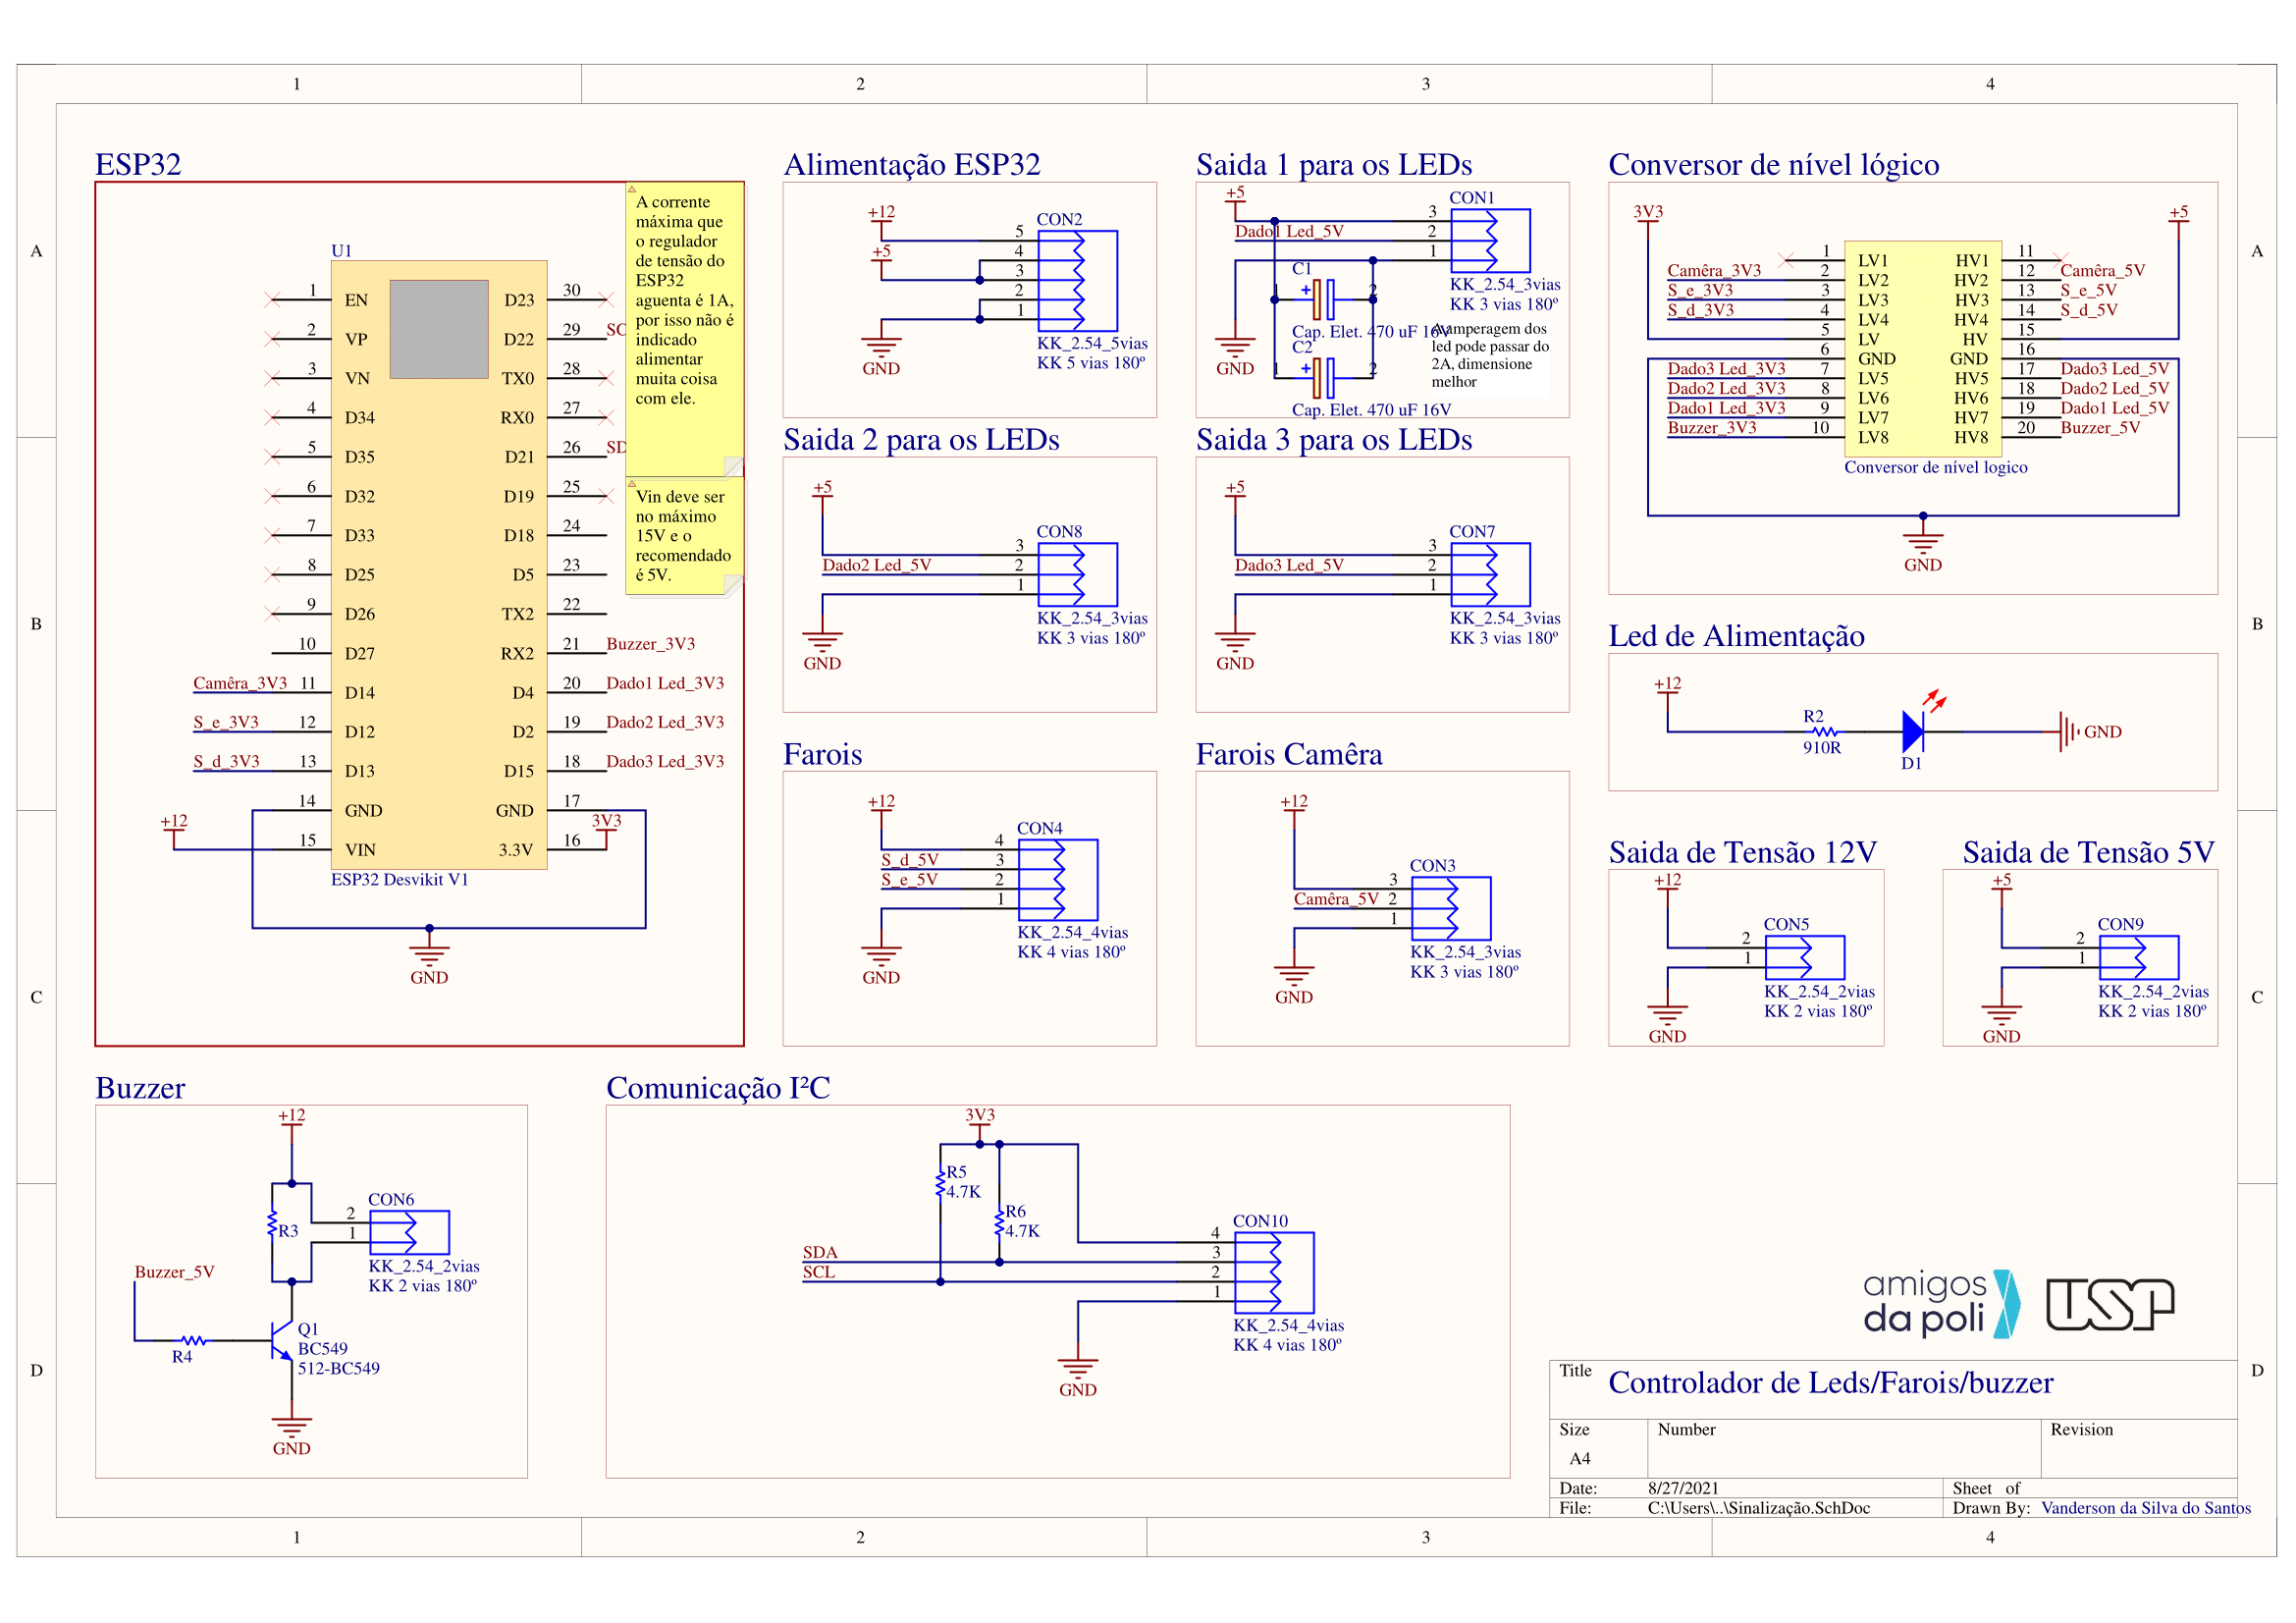
\includegraphics[width=17cm]{modulos/Sinalização-1.png}
    \caption*{Fonte: Elaborado pelo autor no software Altium Design\cite{altium21} }
    \label{Protótipo placa de ## - Esquemático principal}
\end{figure}

Para design do hardware do módulo de Sinalização foi utilizado o CAD e software Altium Designer 21 \cite{altium21} a partir de uma licença estudantil. O projeto completo está disponibilizado em \cite{github_modulos} e todos os componentes usado nesse protótipo podem ser visto na tabela ~\ref{table:Componentes Utilizados na placa de Sinalização - Protótipo}.

\begin{table}[!h]
\caption{Componentes Utilizados na placa de Sinalização - Protótipo}
\centering
\begin{adjustbox}{width=\columnwidth,center}
\begin{tabular}{|c|c|c|c|c|}
\hline
Component                   & Description                                                    & Designator               & Footprint                   & Quantity \\ \hline
Conversor de   nível logico & Conversor de nível   lógico                                    & U2                       & Conversor de nível   lógico & 1        \\ \hline
Cap. Elet. 470   uF 16V     & Aluminum Organic   Polymer Capacitors 16volts 470uF ESR 10mohm & C1, C2                   & Cap. Elet. 470uF 16V        & 2        \\ \hline
KK\_2.54\_3vias             & Conector KK 2.54mm 3   vias                                    & CON1, CON3, CON7,   CON8 & KK\_3vias\_180º             & 4        \\ \hline
KK\_2.54\_5vias             & Conector KK 2.54mm 5   vias                                    & CON2                     & KK\_5vias\_180°             & 1        \\ \hline
KK\_2.54\_4vias             & Conector KK 2.54mm 4   vias                                    & CON4, CON10              & KK\_4vias\_180°             & 2        \\ \hline
KK\_2.54\_2vias             & Conector KK 2.54mm 2   vias                                    & CON5, CON6, CON9         & KK\_2VIAS\_180º             & 3        \\ \hline
LED 5MM RED                 & LED 5MM RED                                                    & D1                       & LED 5MM RED                 & 1        \\ \hline
BC549                       & TRANS NPN 30V 0.1A   TO-92                                     & Q1                       & TO92                        & 1        \\ \hline
RES 470R 1/4W   CARBON FILM & RES 470R OHM 1/4W 5\%   CARBON FILM                            & R2                       & RES 470R 1/4W CARBON   FILM & 1        \\ \hline
RES 1/4W   CARBON FILM      & RES ? OHM 1/4W 5\%   CARBON FILM                               & R3, R4                   & RES 10K 1/4W CARBON   FILM  & 2        \\ \hline
4.7K                        & RES 4.7K OHM 1/4W 5\%   CARBON FILM                            & R5, R6                   & RES 4.7K 1/4W CARBON   FILM & 2        \\ \hline
microcontrolador            & microcontrolador com   moculo bluethoth e wifi                 & U1                       & ESP32\_Desvikit\_v1         & 1        \\ \hline

\end{tabular}
\end{adjustbox}
\centering
\caption*{Fonte: Elaborado pelo autor}
\label{table:Componentes Utilizados na placa de Sinalização - Protótipo}
\end{table}

Dentre os componentes usados, destaca-se os conversores de nível lógico bidirecional, sendo que cada conversor é um módulo com 8 transistores BSS138 \cite{BSS138_datasheet} . Além disso, como já mencionado antes, também usamos o ESP32 \cite{esp32} como microcontrolador do módulo.

%------------------------------------------
\begin{wrapfigure}{r}{5.5cm}
\centering
\caption{ Sensor de distância vl53l0x}\label{wrap-fig:1}
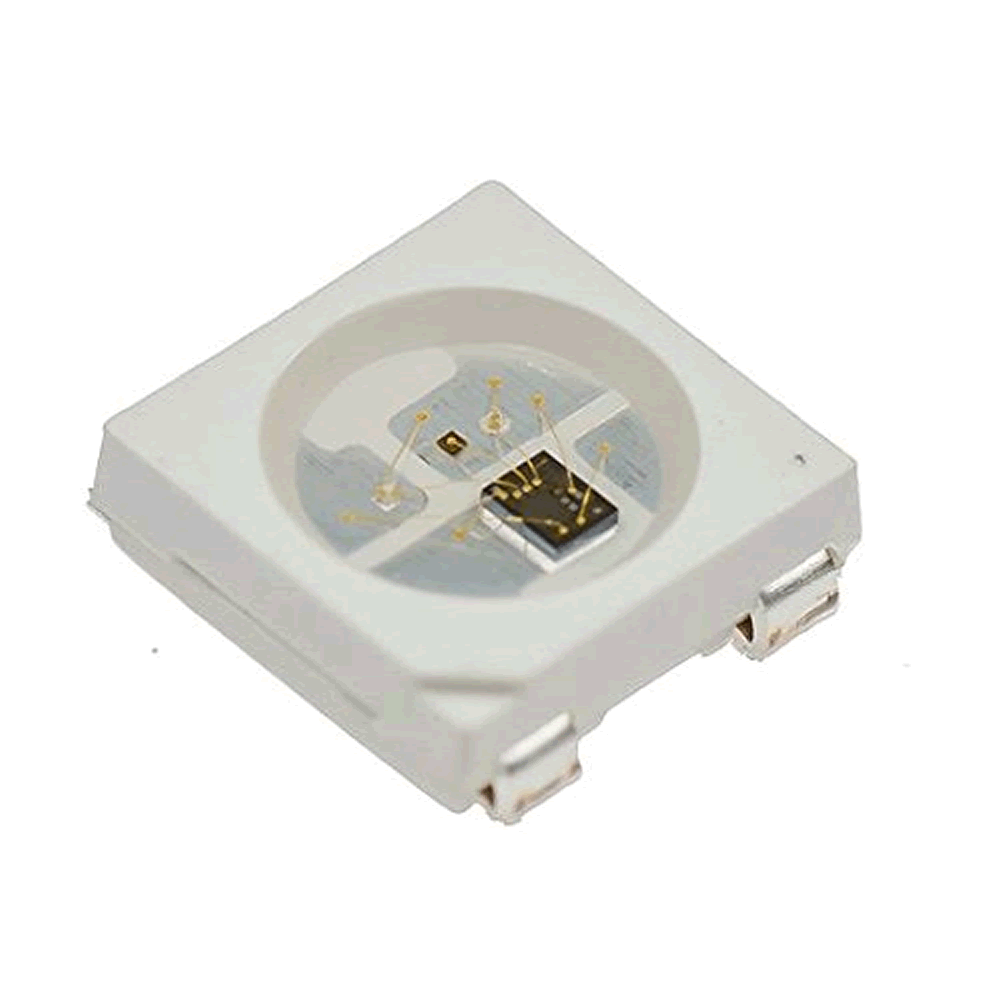
\includegraphics[width=4cm]{modulos/led_rgb_end.png}
\caption*{Fonte: Foto disponibilizada por botnroll}\label{wrap-fig:1}
\end{wrapfigure} 
%------------------------------------------

Para a iluminação do robô, foram escolhidos os leds rgb endereçável ws2812b \cite{WS2812B_datasheet}, que, com um conjunto de três fitas com 80 leds em casa, iluminam o robô por completo. Além disso, para enviar sinais mais de sinalização, foram usados 4 strobos automotivos Ajk 4 \cite{strobos_datasheet}.


\begin{figure}[!ht]
    \centering
    \begin{minipage}{0.5\textwidth}
        \centering
        \caption{Protótipo Sinalização - PCB 2D}
        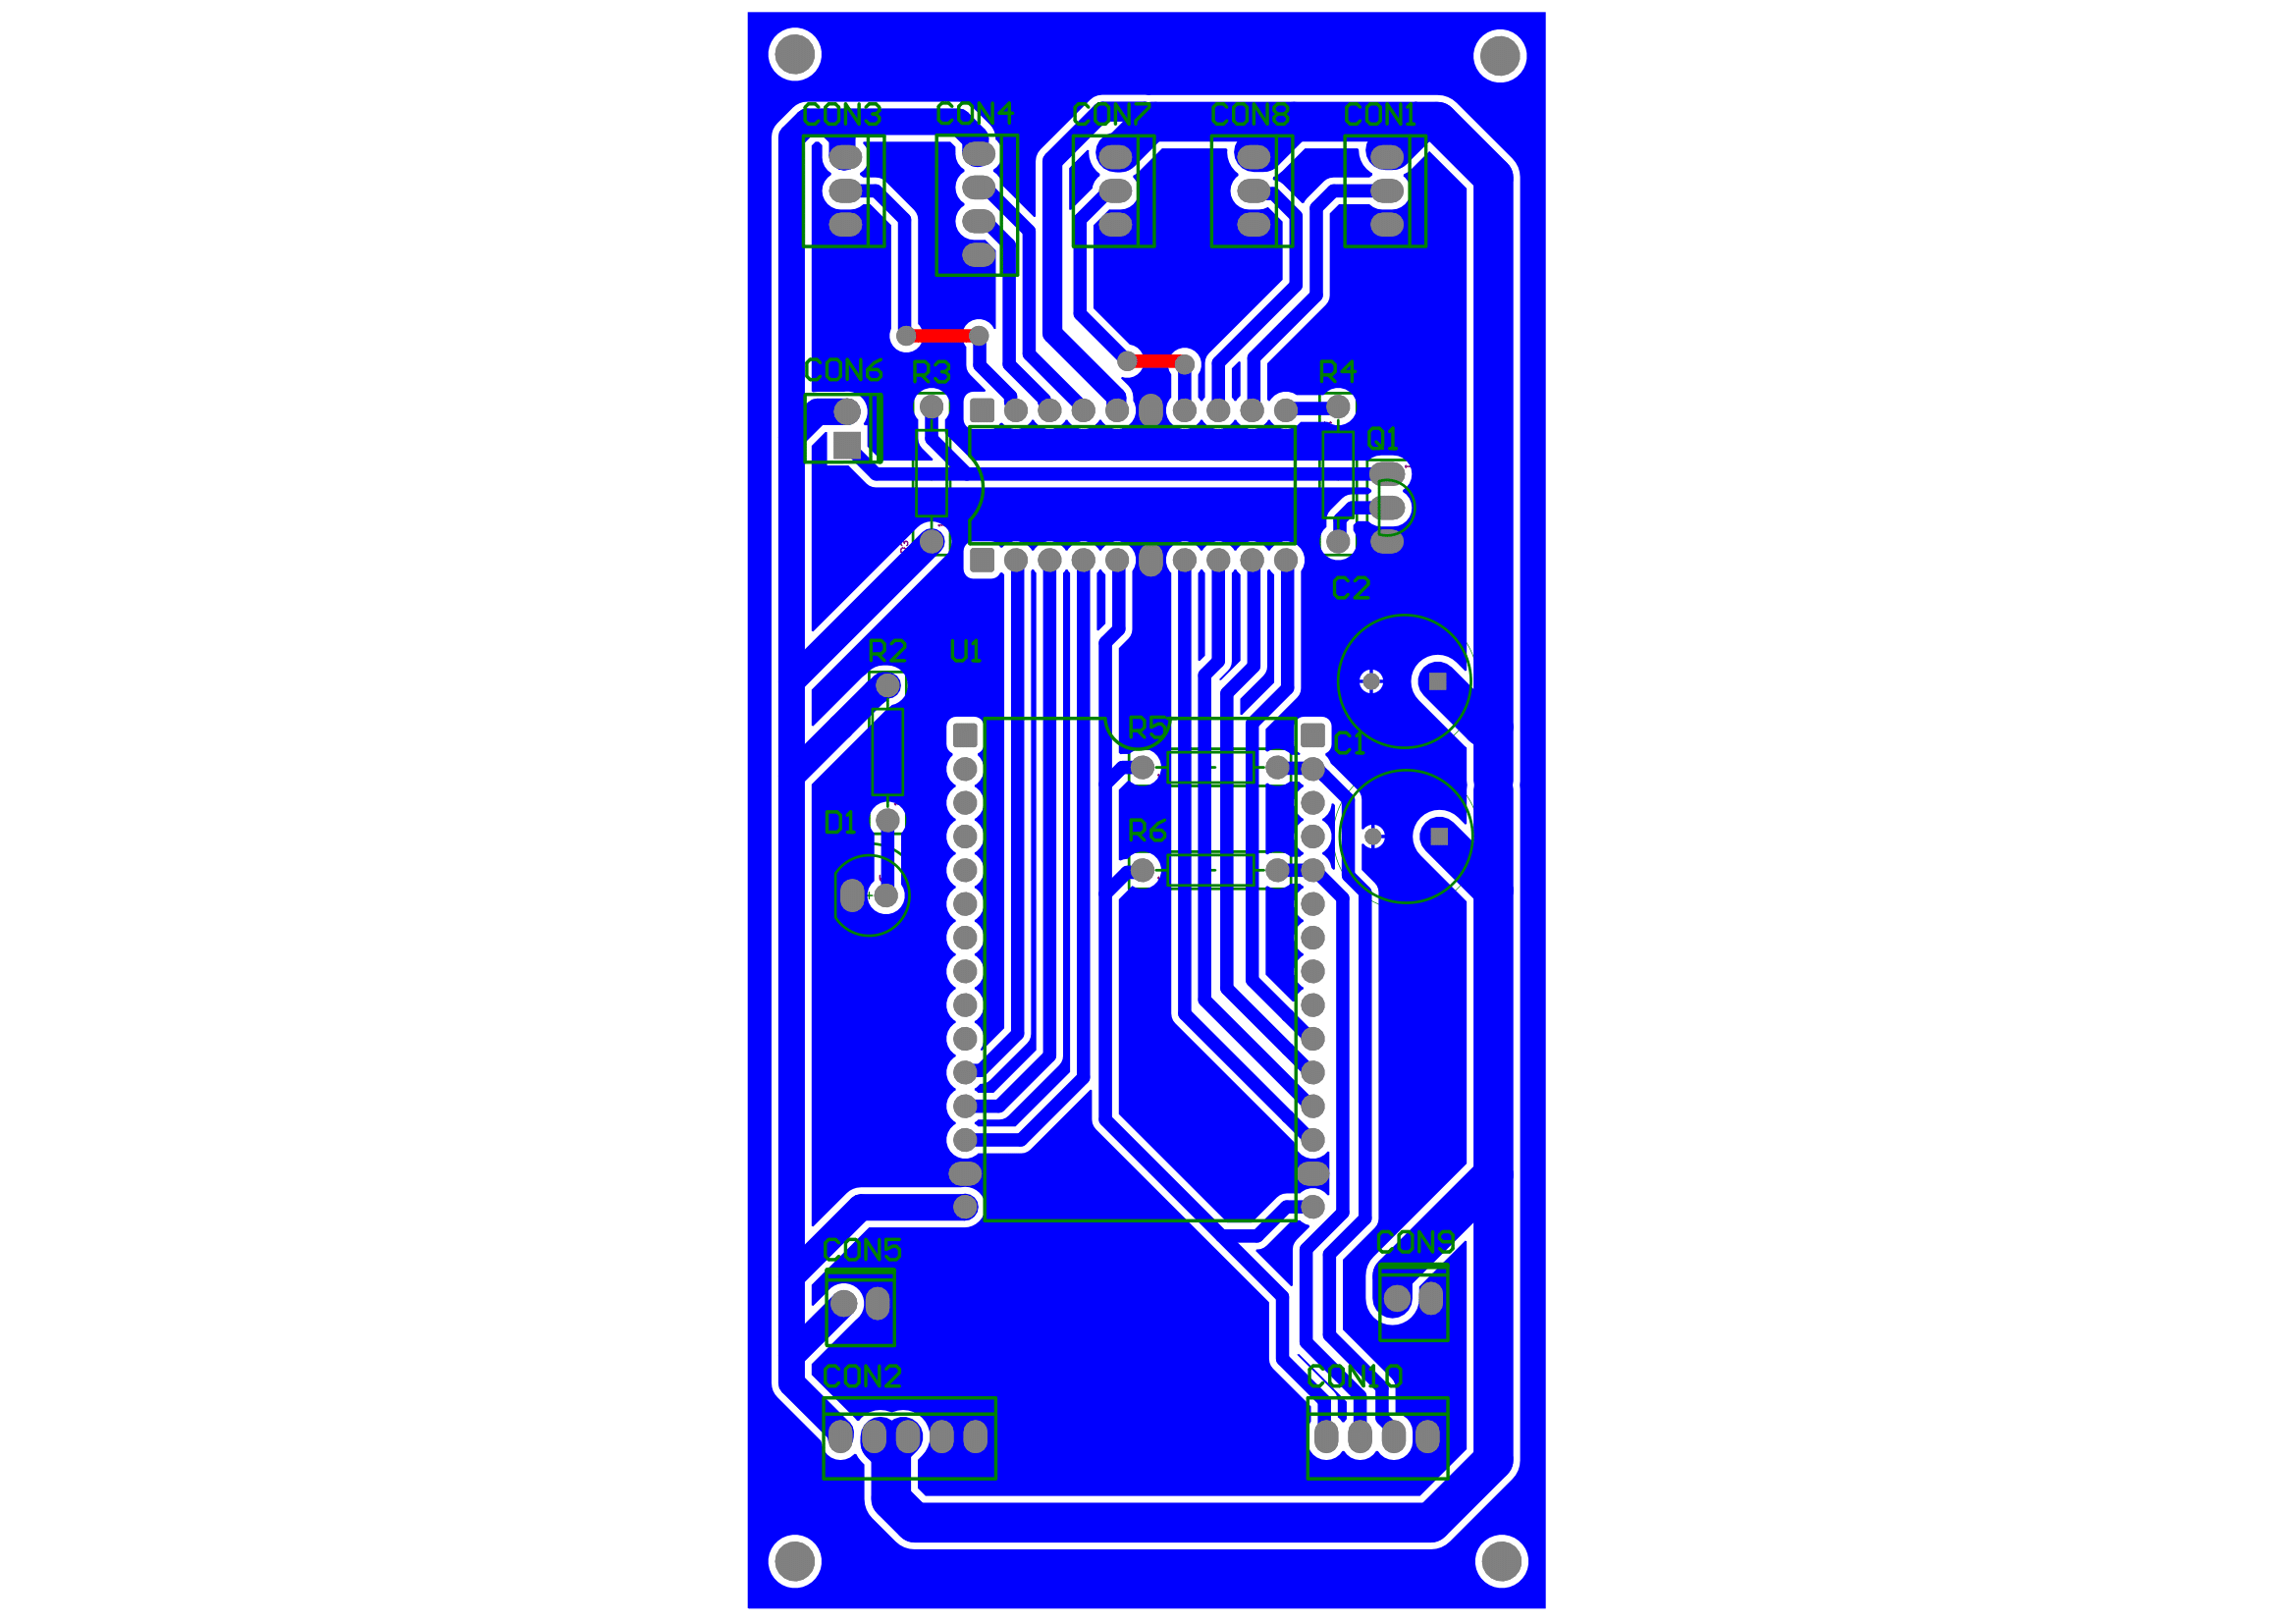
\includegraphics[width=1.03\textwidth]{modulos/Sinalização-2.png} 
        \label{Protótipo Sinalização - PCB 2D}
    \end{minipage}\hfill
    \begin{minipage}{0.5\textwidth}
        \centering
        \caption{Protótipo Sinalização - PCB 3D }
        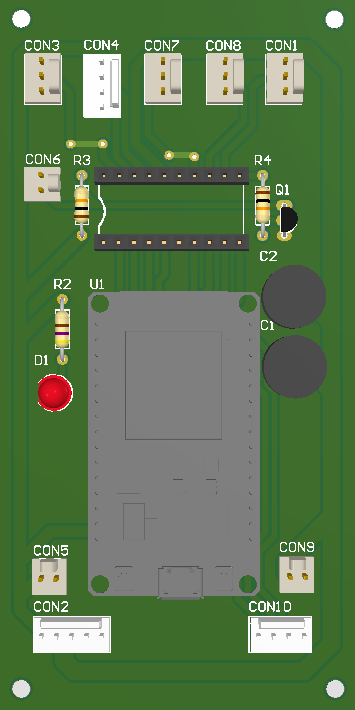
\includegraphics[width=0.4\textwidth]{modulos/Sinalização.png} 
        \label{Protótipo Sinalização - PCB 3D}
    \end{minipage}\hfill
    
    \caption*{Fonte: Elaborado pelo autor no software Altium Design\cite{altium21} }
    \label{fig:Protótipo Sinalização - PCB 2D3D}
\end{figure}

A partir do esquema elétrico que foi feito e do desenho da PCB, a placa de circuito impresso, em uma única camada (Single Layer) e dimensões de 120x60mm. As visões 2D e 3D podem ser vista na figura ~\ref{Protótipo Sinalização - PCB 2D} e ~\ref{Protótipo Sinalização - PCB 3D}.

\begin{comment}
\begin{figure}[!ht]
    \centering
    \begin{minipage}{0.5\textwidth}
        \centering
        \caption{Protótipo Sinalização - Trilhas}
        \includegraphics[width=0.8\textwidth]{example-image-a} 
        \label{fig:figura1minipg}
    \end{minipage}\hfill
    \begin{minipage}{0.5\textwidth}
        \centering
        \caption{Protótipo Sinalização - Completa }
        \includegraphics[width=0.8\textwidth]{example-image-a} 
        \label{fig:figura1minipg}
    \end{minipage}\hfill
    
    \caption*{Fonte: Elaborado pelo autor }
    \label{fig:Protótipo Sinalização - TrilhasC}
\end{figure}
\end{comment}

%================================ SINALIZAÇÂO OfICIAL ========================
\clearpage
\subsubsection{Oficial}

A placa oficial de Sinalização ainda não foi fabricada. Por se tratar de uma placa mais profissional, ela será mandada para ser feita para uma empresa privada ainda não escolhida, não na própria Universidade São Paulo. Assim como o protótipo, o projeto como um todo foi dividido em um esquemático e uma PCB.

\begin{figure}[!h]
\centering
    \caption{placa de Sinalização - Esquemático principal }
    \centering % para centralizarmos a figura
    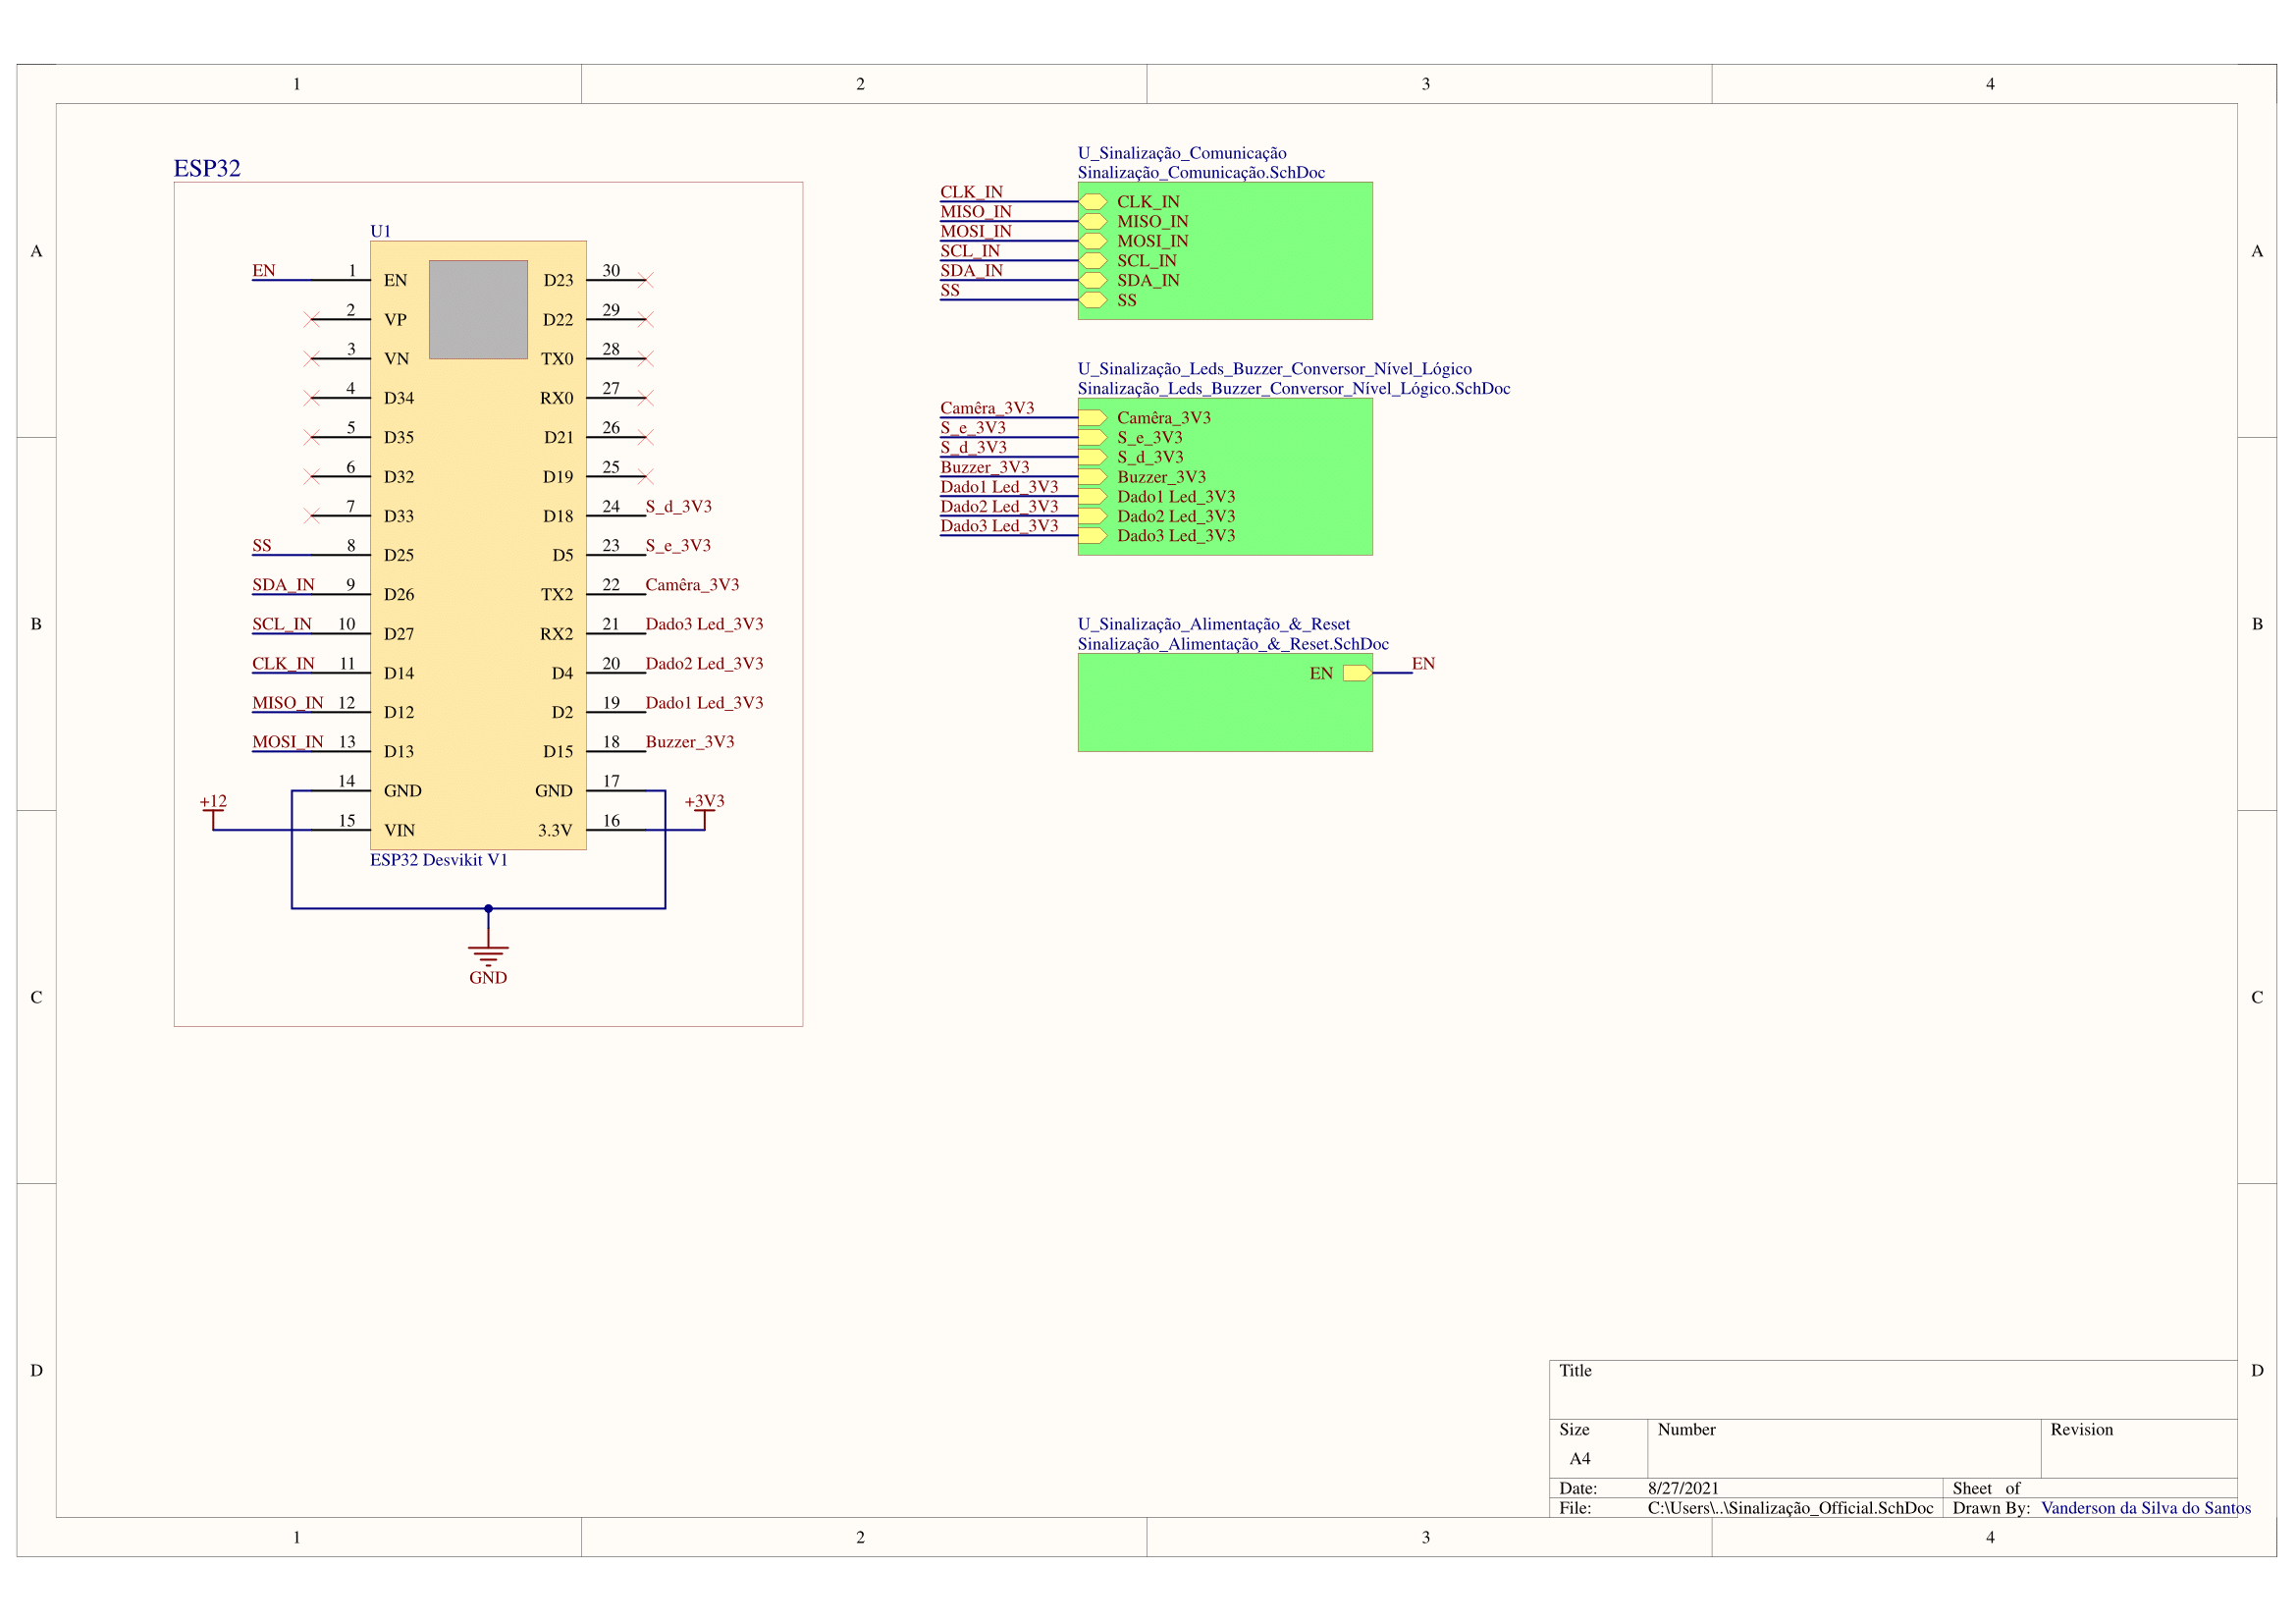
\includegraphics[width=17cm]{modulos/Sinalização_Official-1.png}
    \caption*{Fonte: Elaborado pelo autor no software Altium Design\cite{altium21} }
    \label{Protótipo placa de ## - Esquemático principal}
\end{figure}

Para design do hardware do módulo de Sinalização foi utilizado o CAD e software Altium Designer 21 \cite{altium21} a partir de uma licença estudantil. O projeto completo está disponibilizado em \cite{github_modulos} e todos os componentes usado nessa versão oficial podem ser visto na tabela ~\ref{table:Componentes Utilizados na placa de Sinalização}.

\begin{table}[!ht]
\caption{Componentes Utilizados na placa de Sinalização}
\centering
\begin{adjustbox}{width=\columnwidth,center}
\begin{tabular}{|c|c|c|c|c|}
\hline
Comment                   & Description                                  & Designator                & Footprint                 & Quantity \\ \hline
1000uF 50V                & Capacitor Eletrolitico 1000uF 50V            & C1, C2, C3                & CAPPRD500W62D1300H2650    & 3        \\ \hline
KK\_2.54\_5vias           & Conector KK 2.54mm 5 vias                    & CON1                      & KK\_5vias\_180°           & 1        \\ \hline
KK\_2.54\_4vias           & Conector KK 2.54mm 4 vias                    & CON2, CON7                & KK\_4vias\_180°           & 2        \\ \hline
KK\_2.54\_2vias           & Conector KK 2.54mm 2 vias                    & CON3, CON9, CON11, CON12  & KK\_2VIAS\_180º           & 4        \\ \hline
KK\_2.54\_3vias           & Conector KK 2.54mm 3 vias                    & CON4, CON5, CON6, CON8    & KK\_3vias\_180º           & 4        \\ \hline
KK\_2.54\_6vias           & Conector KK 2.54mm 6 vias                    & CON10                     & KK\_6vias\_180°           & 1        \\ \hline
LED 3MM RED               & LED 3MM RED                                  & D1                        & LED RED                   & 1        \\ \hline
Trans BC817               & Transistor BJT NPN BC817-25-7-F              & Q1, Q2                    & SOT96P240X110-3N          & 2        \\ \hline
4K7                       & Resistor                                     & R1, R2                    & RESC3216X60N              & 2        \\ \hline
1K                        & Resistor                                     & R3                        & RESC3216X60N              & 1        \\ \hline
2K2                       & Resistor                                     & R4, R7                    & RESC3216X60N              & 2        \\ \hline
680R                      & Resistor                                     & R5                        & RESC3216X60N              & 1        \\ \hline
Resistor 1206             & Resistor                                     & R6                        & RESC3216X60N              & 1        \\ \hline
microcontrolador          & microcontrolador com moculo bluethoth e wifi & U1                        & ESP32\_Desvikit\_v1       & 1        \\ \hline
Conversor de nível logico & U2                                           & Conversor de nível lógico & Conversor de nível logico &          \\ \hline

\end{tabular}
\end{adjustbox}
\centering
\caption*{Fonte: Elaborado pelo autor}
\label{table:Componentes Utilizados na placa de Sinalização}
\end{table}

Em relação ao protótipo, pouco mudou da lógica por trás do circuito, a principal diferença é que o modelo oficial utiliza todos componentes com encapsulamento SMD \cite{SMD_def}. Além disso, foi adicionado o protocolo de comunicação SPI também, como já foi comentado no início do capítulo.

\begin{figure}[!h]
    \centering
    \begin{minipage}{0.5\textwidth}
        \centering
        \caption{Sinalização - PCB 2D}
        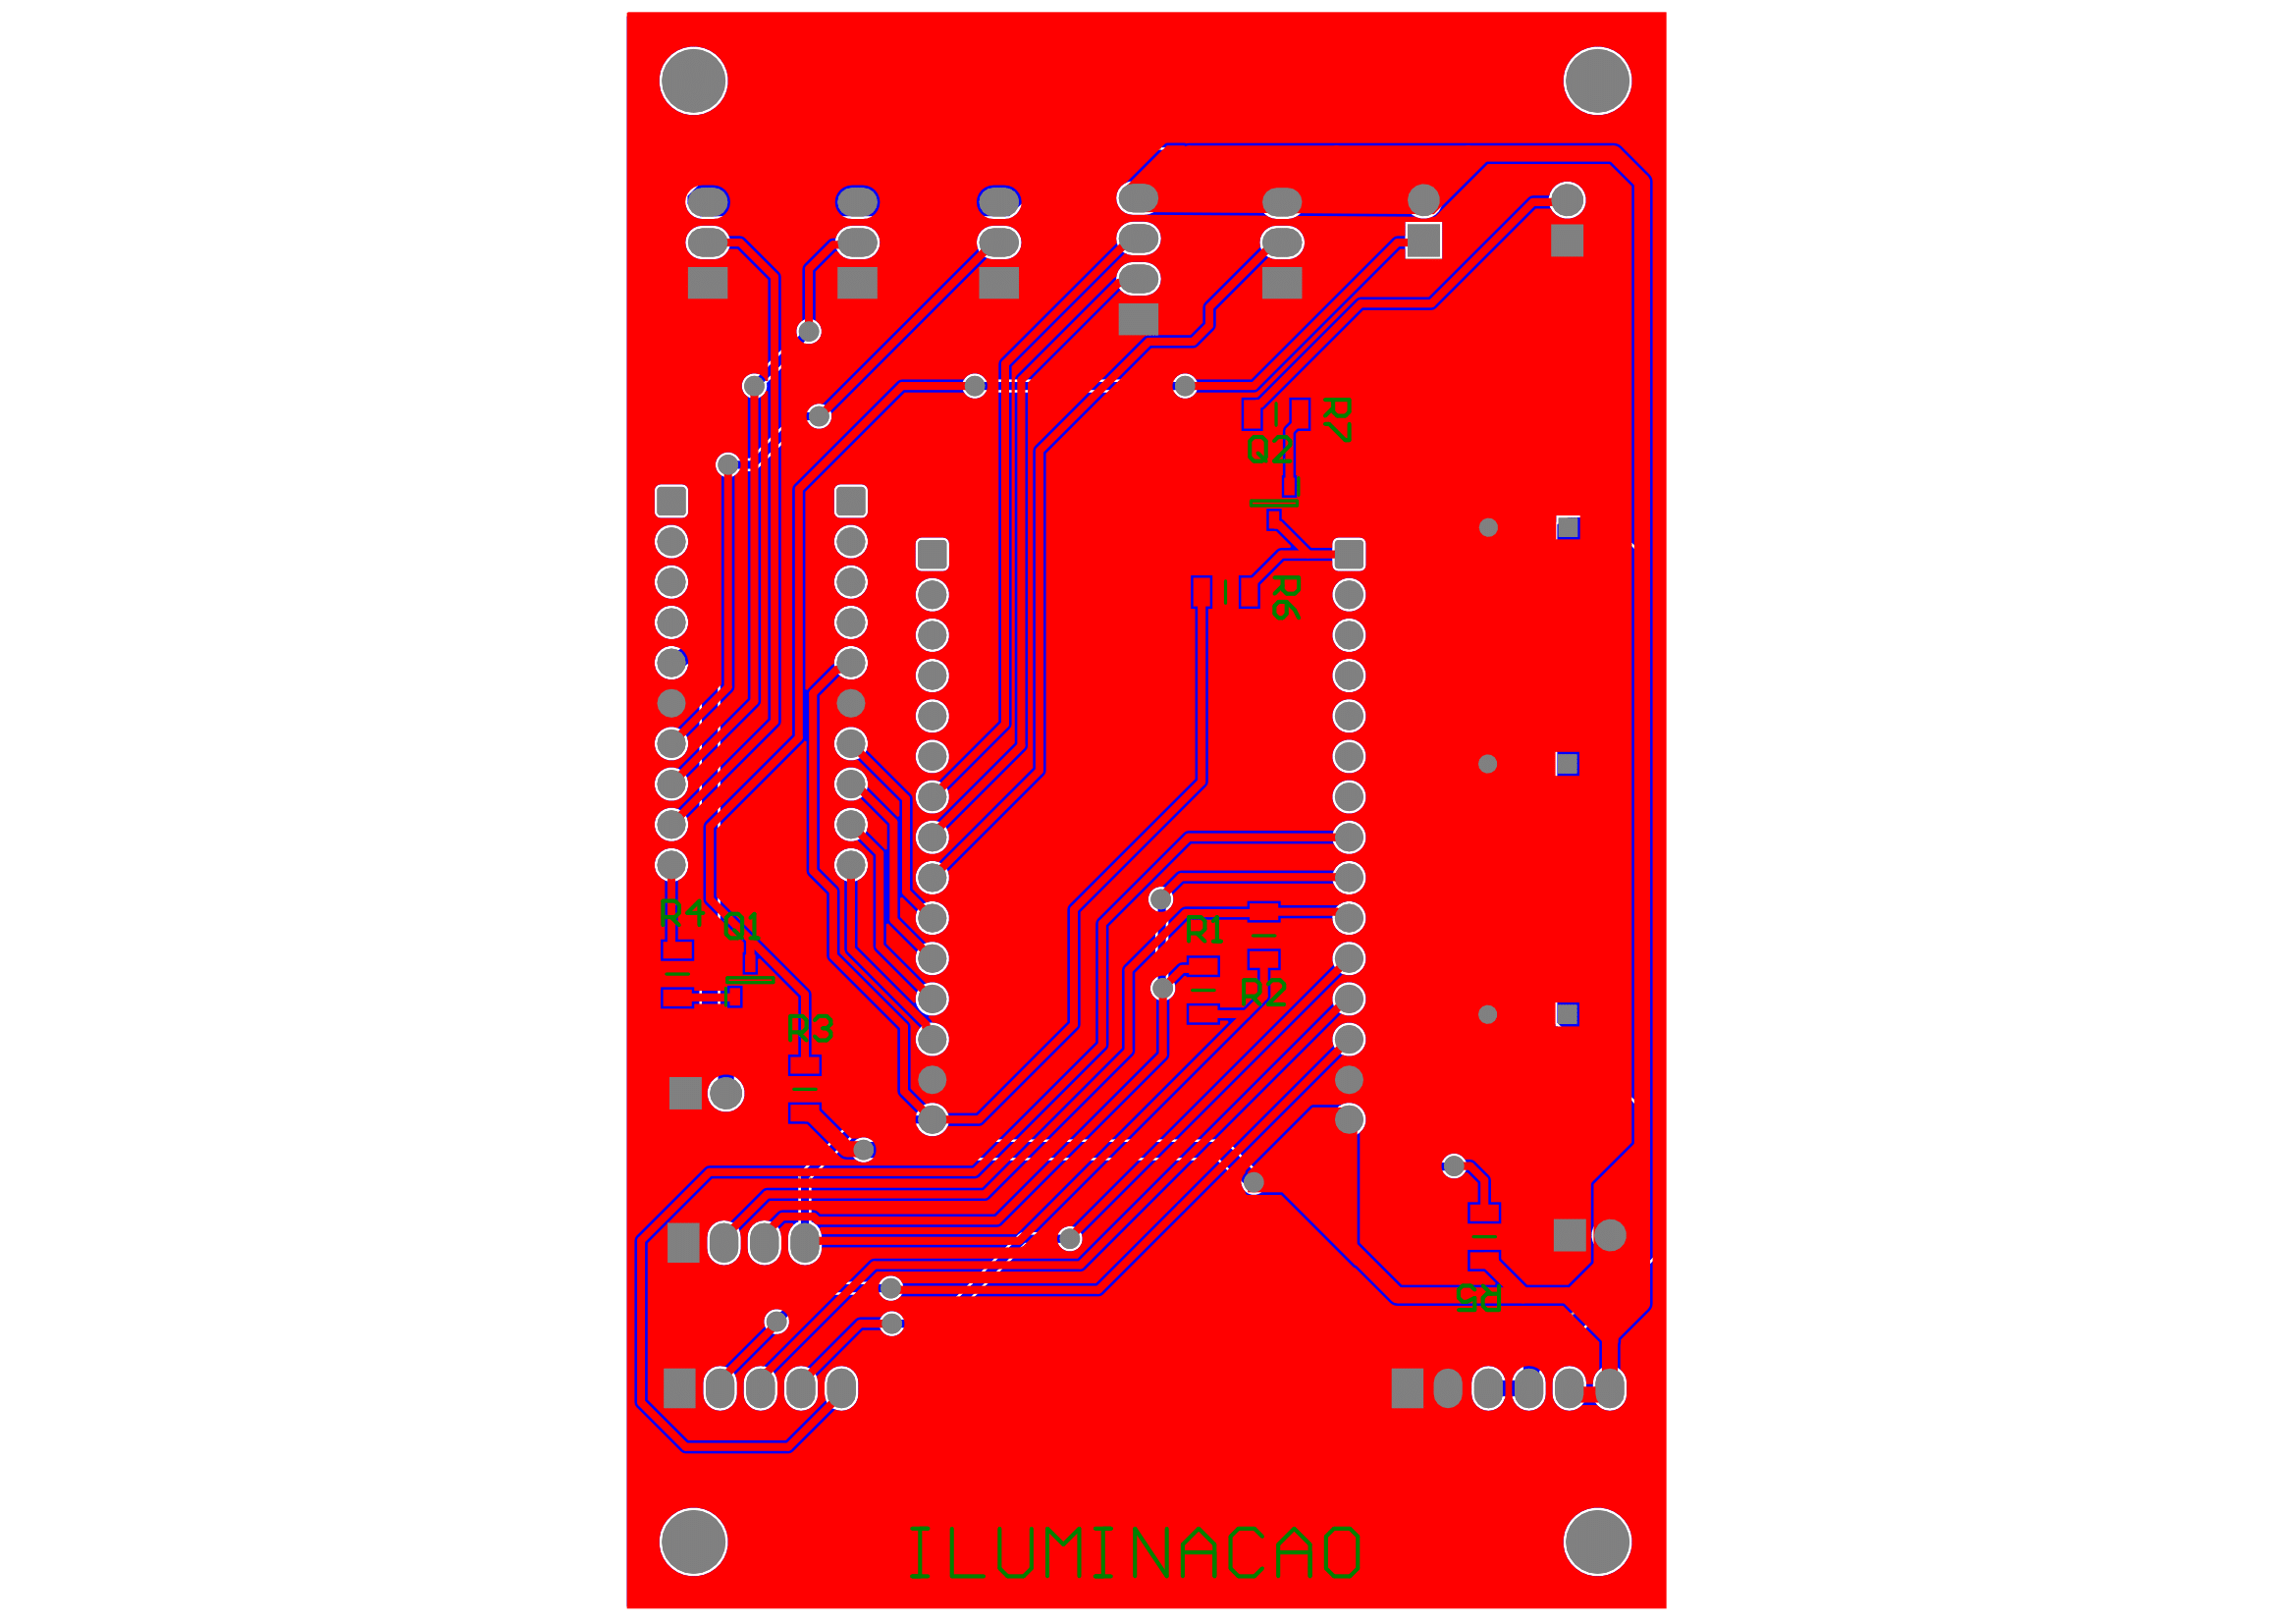
\includegraphics[width=1.03\textwidth]{modulos/Sinalização_Official-5.png} 
        \label{fig:figura1minipg}
    \end{minipage}\hfill
    \begin{minipage}{0.5\textwidth}
        \centering
        \caption{Sinalização - PCB 3D }
        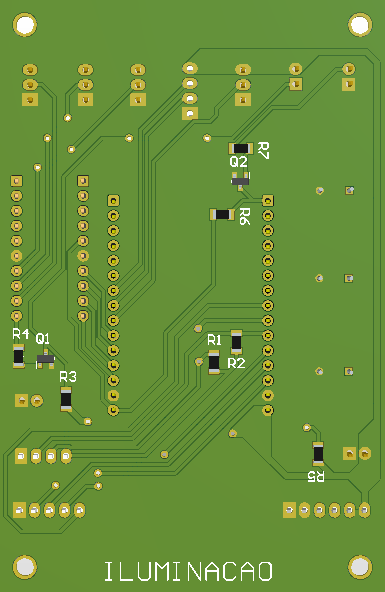
\includegraphics[width=0.5\textwidth]{modulos/Sinalização_Official.png} 
        \label{fig:figura1minipg}
    \end{minipage}\hfill
    
    \caption*{Fonte: Elaborado pelo autor no software Altium Design\cite{altium21} }
    \label{fig:Sinalização - PCB 2D3D}
\end{figure}

A placa de circuito impresso está completa, porém ainda não foi feito o pedido oficial de fabricação.

\begin{comment}
%================================ SINALIZAÇÂO FIRMWARE ========================
\subsection{Firmware}
\end{comment}
\end{document}